\documentclass[11pt]{beamer}

\beamertemplatenavigationsymbolsempty 

\usepackage{tikz}
\usetikzlibrary{positioning,shapes,matrix,arrows}

\usepackage[default]{gfsneohellenic}
\usepackage[LGR,T1]{fontenc}

\usepackage[ruled,vlined]{algorithm2e}
\usepackage{extarrows}
\usepackage{graphicx}
\usepackage{latexsym}
\usepackage{amsmath, amssymb, amsfonts, amsthm}
\usepackage{amsmath,amsthm,verbatim,amssymb,amsfonts,amscd, graphicx}
\usepackage{mathtools}
\usepackage{color}
\graphicspath{{./figs/}} %note trailing /
\setbeamertemplate{footline}{\insertpagenumber / \insertdocumentendpage}
\usepackage{times}
%\usefonttheme{serif}

\usepackage{tikz}
\usetikzlibrary{shapes.arrows}


\tikzset{
    myarrow/.style={
        draw,
        fill=orange,
        single arrow,
        minimum height=3.5ex,
        single arrow head extend=1ex
    }
}
\newcommand{\arrowup}{%
\tikz [baseline=-0.5ex]{\node [myarrow,rotate=90] {};}
}
\newcommand{\arrowdown}{%
\tikz [baseline=-1ex]{\node [myarrow,rotate=-90] {};}
}



\def\R{{\mathbb R}}
\def\Q{{\mathbb Q}}
\def\Z{{\mathbb Z}}
\def\N{{\mathbb N}}
\def\C{{\mathbb C}}
\def\E{{\mathbb E}}
\def\R{{\mathbb R}}
\def\Y{{\mathcal Y}}
\def\L{{\mathcal L}}
\def\H{{\mathcal H}}
\def\D{{\mathcal D}}
\def\P{{\mathbb P}}
\def\M{{\mathbb M}}
\def\S{{\mathbb S}}
\def\A{{\mathbf A}}
\def\x{{\mathbf x}}
\def\b{{\mathbf b}}
\def\a{{\mathbf a}}
\def\Ph{{\mathbf {\Phi}}}

\def\h{{\mathbf{h}}}
\def\G{{\Gamma}}
\def\s{{\sigma}}
\def\e{{\varepsilon}}
\def\l{{\lambda}}
\def\p{{\phi}}
\def\v{{\mathbf{v}}}
\def\t{{\theta}}
\def\z{{\zeta}}
\def\o{{\omega}}
\def\y{{\mathbf{y}}}
\def\g{{\mathbf{g}}}
\def\u{{\mathbf{u}}}
\def\w{{\mathbf{w}}}


%\usepackage{algorithm}
%\usepackage{algorithmic}

\usepackage{multimedia}

\title{Analysis of The Ratio of $\ell_1$ and $\ell_2$ Norms in Compressed Sensing}
\author{Yiming Xu 
\\ \ \\ \ Department of Mathematics
\\ \ \\ \  University of Utah\\ \ \\ \
}



\vspace{6cm}

\date{}


\begin{document}
\begin{frame}
  \titlepage 
\end{frame}

\begin{frame}
\frametitle{Introduction}
\begin{itemize}
\item $\x\in\R^n$: An $n$-dimensional signal
\item $\A\in\R^{m\times n}$: A measurement matrix with $m$ linear measurements
\item $\b\in\R^m$: The values of $m$ linear measurements
\end{itemize}

\bigskip 

\begin{center}

Goal: Reconstruct $\x$ from the pair $(\A, \b)$, when $m\ll n$. 
\end{center}

\end{frame}


\begin{frame}
\frametitle{An underdetermined system}

\begin{itemize}
\item If $\A$ has full row rank, then $\A\x=\b$ has infinitely many solutions.

\item Additional constraint needs to be imposed to make the solution unique. 

\item In the context of signal processing, the constraint is the {\color{red}sparsity} of $\x$. 
\end{itemize} 


\medskip

These are the basic ideas behind a new modality in modern signal processing, called \emph{Compressed Sensing}, or CS.  



\end{frame}

\begin{frame}
\frametitle{Mathematical formulation}
\centering

The CS problem can be mathematically formulated as a combinatorial optimization problem:
\begin{align*}
\min_{\x}||\x||_0\ \ \ \text{subject to}\ \A\x=\b, 
\end{align*}
where $|| \cdot||_0$ is the sparsity measure defined by
\begin{align*}
||\x||_0:=\lim_{q\rightarrow 0}||\x||_q^q=|\{i\leq n, x_i\neq 0\}|.
\end{align*}


\end{frame}

\begin{frame}
\frametitle{A sufficient condition \footnote{Donoho et al., PNAS, 2003} for well-definedness}

\begin{Definition}[Donoho, Elad]
The \emph{spark} of a matrix $\A$ is the smallest number of columns from $\A$ that are linearly-dependent. 
\end{Definition}

\medskip

\begin{Theorem}[Donoho, Elad]
Let $\x_0$ be an $s$-sparse solution to $\A\x=\b$. Then, $\x_0$ is the unique minimizer to the CS optimization problem if $spark(\A)>2s$. 
\end{Theorem}

\medskip

\begin{itemize}
\item This Theorem is a analogous to the \emph{Uncertainty Principle} in harmonic analysis.
\item $\text{Spark}(\A)\leq m+1$. Equality holds in many cases of interest.  
\end{itemize} 

\end{frame}



\begin{frame}
\frametitle{How to find the solution?}

Two classical approaches:

\begin{itemize}
\item Orthogonal Matching Pursuit (OMP)
[{\color{blue} \it Gilbert and Tropp, IEEE Trans. on Info. Theory, 2004}]

\begin{itemize}
\item Greedy algorithm in nature
\item Fast and transparent
\item Non-uniform recovery
\end{itemize}  

\medskip

\item Basis Pursuit (BP) [{\color{blue} \it Donoho; \it Cand\`es et al., IEEE Trans. on Info. Theory, 2006}]
\begin{itemize}
\item Relaxation scheme
\item Linear programming computational cost
\item Uniform recovery
\end{itemize} 
\end{itemize}



\end{frame}


\begin{frame}
\frametitle{A closer look at BP}

\begin{align*}
\text{CS}:\ \ \ \min_{\x}||\x||_0\ \ \ \text{subject to}\ \A\x=\b, 
\end{align*}
\begin{center}
\begin{tabular}{rc}
\arrowdown\\[1ex]
\end{tabular}
\end{center}
\begin{align*}
\text{BP}:\ \ \ \min_{\x}||\x||_{\color{red}1}\ \ \ \text{subject to}\ \A\x=\b, 
\end{align*}

\medskip

$\ell_1$ norm as objective function:
\begin{itemize}
\item Sparsity-promoting
\item Convex optimization
\end{itemize} 

\end{frame}


\begin{frame}
\frametitle{Equivalence between CS and BP\footnote{Cohen et al., JAMS, 2009}}

\begin{definition}[Cohen et al.]
$\A\in\R^{m\times n}$ is said to satisfy the null space property (NSP) with parameters $(s, c)$ if 
\begin{align*}
||\h_T||_1< c||\h_{T^c}||_1\ \ \ \forall \h\in\ker(\A), 
\end{align*}
and $T\subset\{1,\cdots, n\}$ with $|T|\leq s$.  
\end{definition}

\medskip

\begin{theorem}[Cohen et al.]
CS $\Leftrightarrow$ BP for all $s$-sparse vectors if $\A$ satisfies NSP with parameters $(s,1)$. On the other hand, that $\A$ satisfies NSP with parameters $(2s,1)$ is necessary for CS $\Leftrightarrow$ BP for all $s$-sparse vectors. 
\end{theorem} 


\end{frame}



\begin{frame}
\frametitle{A sufficient condition\footnote{Cand\`es and Tao, IEEE Trans. on Info. Theory, 2006} for NSP}

\begin{definition}[Cand\`es and Tao]
$\A\in\R^{m\times n}$ is said to satisfy the restricted isometry property with parameters $(s, \delta)$ if for any $S\subset\{1, \cdots, n\}$ with $|S|= s$, the restriction of $\A$ to $T$ satisfies
\begin{align*}
(1-\delta)||\x||^2_2\leq ||\A_S\x||^2_2\leq (1+\delta)||\x||^2_2, \ \ \ \forall\x\in\R^s. 
\end{align*}
\end{definition}

\begin{theorem}[Cand\`es and Tao]
\begin{center}
RIP with parameters $(2s, \frac{1}{3})$ $\Rightarrow$ NSP with parameters $(s, 1)$. 
\end{center}
\end{theorem} 

\medskip

{\color{orange}Remark}: RIP is strictly stronger than NSP. 
\end{frame}

\begin{frame}
\frametitle{Practicality of RIP\footnote{Rudelson and vershynin, CPAM, 2008}}

\begin{Theorem}[Rudelson and Vershynin]

Let $\A\in\R^{m\times n}$ be a random matrix. 
\begin{enumerate}

\item If $\A$ is an isotropic subgaussian matrix, $\A/\sqrt{m}$ satisfies RIP with parameters $(s, \delta)$ with high probability if $$m\gtrsim \delta^{-2}{\color{red}s\log\left(\frac{n}{s\delta^2}\right)}.$$

\medskip

\item If $\A$ is a partial bounded orthogonal matrix, $\sqrt{n}\A/\sqrt{m}$ satisfies RIP with parameters $(s, \delta)$ with high probability if $$m\gtrsim \delta^{-2}{\color{red}s\log^5 n}.$$  
\end{enumerate}
\end{Theorem} 
\end{frame}

\begin{frame}
\frametitle{Alternative perspectives on BP}

The BP problem can be studied without using RIP:

\begin{itemize}
\item High-dimensional geometry approach: [{\color{blue}\it Vershynin, Sampling Theory, 2015}]

\medskip

\item Null space ratio: [{\color{blue}\it Zhang, Journal of the Operations Research Society of China, 2013}] 
\end{itemize}


\end{frame} 

\begin{frame}
\frametitle{Is BP always good?}

\begin{itemize}
\item Tanner et al. observed and studied in a series of papers [{\color{blue}\it PNAS, 2005, JAMS, 2009, SIAM Review, 2011}] that $\ell_1$ minimization exhibits a phase transition phenomenon. This implies that $\ell_1$ model fails intrinsically when the sampling rate is lower than some threshold. 

\bigskip

\item Many other relaxation methods, though non-convex in nature, demonstrate better empirical performance than $\ell_1$.  

\end{itemize}

\end{frame}


\begin{frame}
\frametitle{Non-convex relaxation methods}
\begin{itemize}
\item IRLS-$\ell_q$ $(0<q<1)$ [{\color{blue}\it Chartrand, IEEE Signal Process. Lett., 2007, Foucart and Lai, Appl. \& Comp. Harm. Anal., 2009, Daubechies et al., CPAM, 2010}]
\medskip
\item Reweighted $\ell_1$ [{\color{blue}\it Cand\`es et al., Journal of Fourier Anal. \& Appl., 2007}] 
\medskip
\item {\color{orange}CoSaMP} [{\color{blue} \it Needell and Tropp, Appl. \& Comp. Harm. Anal., 2009}]
\medskip
\item {\color{orange}IHT} [{\color{blue} \it Blumensath and Devies, Appl. \& Comp. Harm. Anal., 2009}]
\medskip
\item $\ell_1-\ell_2$ [{\color{blue} \it Yin et al, \& SIAM Journal on Sci. Comp., 2015}]
\end{itemize}
\medskip
\ \ \ \ \ \ \ $\cdots \cdots$
\end{frame}

\begin{frame}
{Model comparison: A numerical example\footnote{Yin et al., SIAM Journal on Sci. Comp., 2015}}
\begin{figure}
\begin{center}
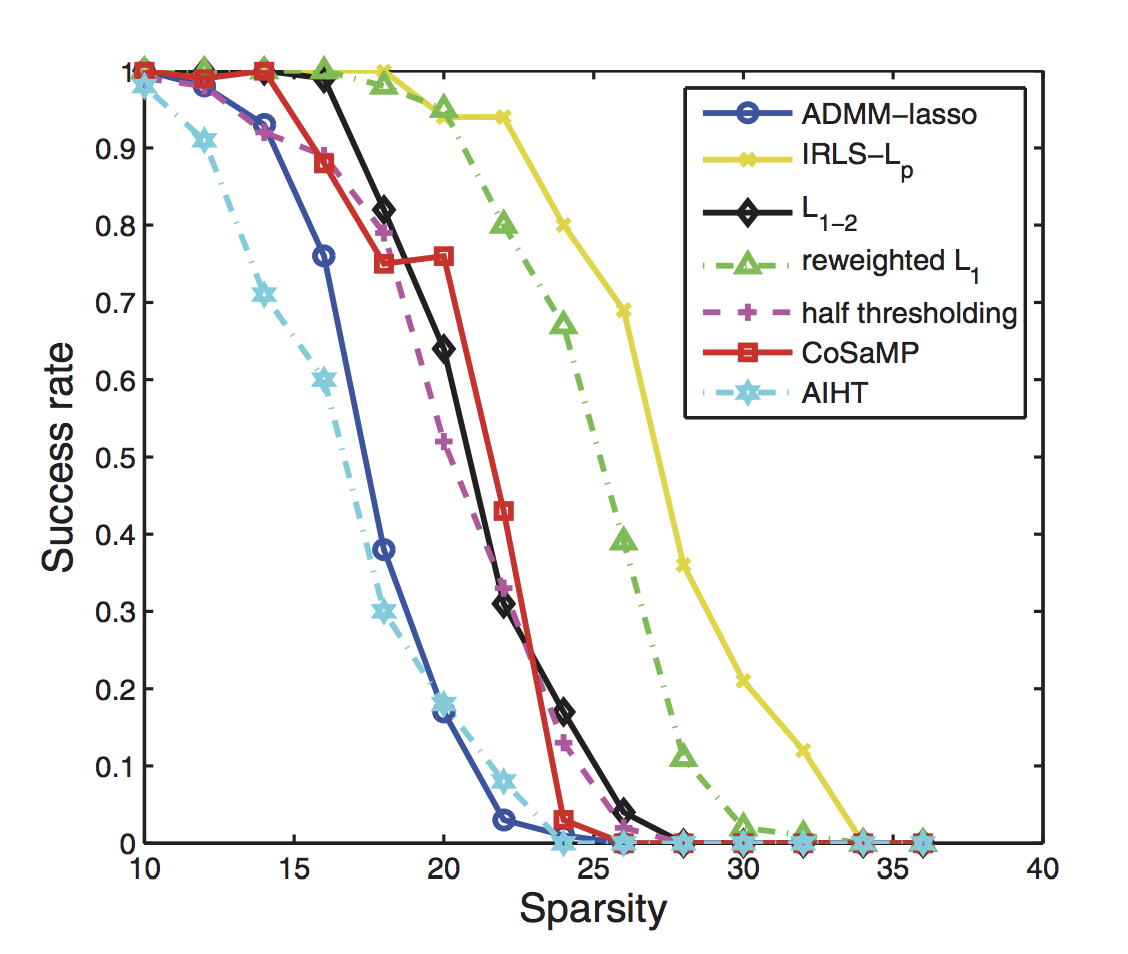
\includegraphics[width=7.8cm]{comparison.png}
\caption{Average recovery rate comparison for $64\times 256$ gaussian random measurements and standard normal coefficients.}
\end{center}
\end{figure}

\end{frame}


\begin{frame}
{An exact recovery condition\footnote{Tran and Webster, Results in Applied Mathematics, 2019} for Non-convex models}

\begin{Theorem}[Tran and Webster]
Consider the general non-convex relaxation problem:
\begin{align*}
\min R(\x) \ \ \ \text{subject to}\ \A\x=\A\x_0,
\end{align*}
where $R:\R^n\rightarrow [0, \infty)$. If $R(\x)$ satisfies
\begin{itemize}
\item (Summetry): $R(\x)=R(|p(\x)|)$ for all $\x\in\R^n$, where $p(\x)$ is any permutation of $\x$. 
\item (Concavity): $R(\x)$ is concave on $[0,\infty)^n$.  
\item (Strict monotonicity): $R(\x)\leq R(\y)$ if $\x\leq \y$ and $\x, \y\geq \mathbf{0}$. The equality holds if and only if $\x=\y$.  
\end{itemize}
Then the NSP condition with parameters $(s,1)$ is sufficient to guarantee recovery of $\x_0$ for all $\x_0$ with $||\x_0||_0\leq s$. 
\end{Theorem}

\end{frame}




\begin{frame}
\frametitle{A scale-invariant relaxation method}
We propose to study a different type of non-convex relaxation methods called ${\color{red}\ell_{q_1}/\ell_{q_2}}$ in CS:
\begin{align*}
\min_{\x}\frac{||\x||_{q_1}}{||\x||_{q_2}}\ \ \ \text{subject to}\ \A\x=\b,
\end{align*}
where $q_1<q_2$. For convenience, we focus on the case $q_1\leq 1$ and $q_2=2$.  
\end{frame}

\begin{frame}
{Why study the ratio?}
\begin{itemize}
\item Scale invariance resembling $|| \cdot||_0$

\item Promote sparsity [{\color{blue} \it Hurley and Rickard, IEEE Trans. on Info. Theory, 2009}]

\begin{figure}
\begin{center}
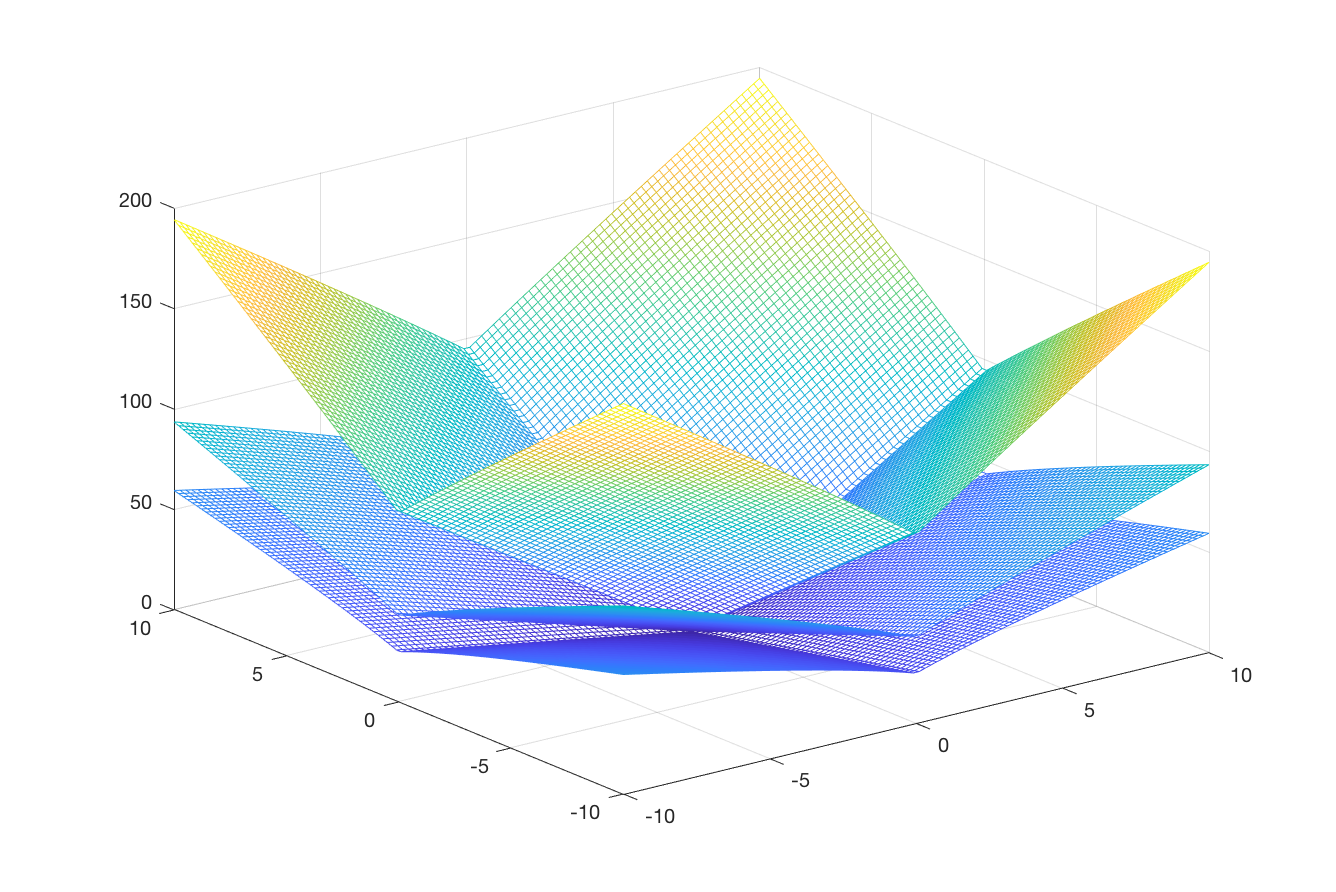
\includegraphics[width=6cm]{levelset.png}
\end{center}
\end{figure}


\item Better empirical performance and admits a multi-dimensional generalization [{\color{blue} \it Petrosyan et al., App. Num. Math., 2019}]


\item {\color{red} Very little theory behind} (To my knowledge) 
\end{itemize}
\end{frame}




\begin{frame}
\frametitle{Related works on $\ell_{q_1}/\ell_{q_2}$} 

\begin{itemize}

\item  
Yin et al. studied $\ell_1/\ell_2$ in [{\color{blue} \it Yin et al., Comm. in Info. Systm., 2014}] in the case of positive sparse recovery. They proposed a sufficient condition for the global optimality of $\x_0$ using the dynamic range of $\x_0$.  

\medskip

\item Rahimi et al. studied $\ell_1/\ell_2$ in [{\color{blue} \it Rahimi et al., arxiv., 2018}] the general case of CS. They proposed a sufficient condition called $s$-NSP for the local optimality of $\x_0$. They also proposed an ADMM-type algorithm to solve $\ell_1/\ell_2$. Furthermore, they introduced a box constraint to improve the performance of the algorithm.   

\medskip

\item Wang et al. studied the algorithmic aspects of $\ell_1/\ell_2$ in [{\color{blue} \it Wang et al., arxiv., 2019}]. They proposed an accelerated scheme to solve $\ell_1/\ell_2$ using a bisection approach. 

\end{itemize}

\end{frame}

\begin{frame}
{Our contributions}


\begin{itemize}

\item  
Give a more interpretable local optimality condition on $\x_0$ in the case of $\ell_1/\ell_2$. (Inspired by {\color{blue} Tran and Webster}) 

\medskip

\item Give the first sufficient condition for exact recovery of $\x_0$ in the case of $\ell_q/\ell_2$ $(q<1)$, and show that the condition is easily satisfied for a large class of random matrices when $q=1$. (Inspired by {\color{blue} Vershynin and Zhang})    

\medskip

\item Provide an elementary analysis on the stability of the $\ell_1/\ell_2$ model. (Inspired by {\color{blue} Zhang}) 

\medskip

\item Propose a support-selection based multi-initialization approach for the current $\ell_1/\ell_2$ algorithm, which further enhances the recovery rate. (Inspired by {\color{red} failures})     

\end{itemize}

\end{frame}


\begin{frame}
\frametitle{$\ell_1/\ell_2$: Local optimality condition}

\begin{Theorem}[Narayan and Xu]
Let $\x_0$ be a nonzero $s$-sparse vector and define
\begin{align*}
\kappa:=\frac{||\x_0||_1||\x_0||_\infty}{||\x_0||^2_2}.
\end{align*}
Suppose that $\x_0$ satisfies  
\begin{align*}
\rho:=\frac{\min_{i\in\text{supp}(\x_0)}|x_i|}{\max_{i\in\text{supp}(\x_0)}|x_i|}\leq\frac{1}{2c(\kappa+1)},
\end{align*}
where $c$ is a parameter decoupled from $\x_0$ defined by 
\begin{align*}
c:=\sup_{\mathbf{0}\neq \h\in\ker(\A)}\frac{||\h||^2_2}{||\h||_1^2}
\end{align*}
If $\A$ satisfies NSP with parameters $(s, \frac{1}{2\kappa+1})$, then $\x_0$ is the local minimizer of $\ell_1/\ell_2$.   
\end{Theorem}

\end{frame}

\begin{frame}
\frametitle{$\ell_1/\ell_2$: Global optimality condition}

\begin{Theorem}[Narayan and Xu]
A sufficient condition for $\ell_q/\ell_2$ ($q<1$) is
\begin{align*}
\inf_{\h\in\ker(\A)-\{\mathbf{0}\}}\frac{||\h||_q}{||\h||_2}>3^{1/q}s^{1/q-1/2}.
\end{align*}
In the case of $q=1$ and $\A$ is an isotropic subgaussian random matrix with independent rows, this condition holds true with probability at least $1-2e^{-u^2}$ if
\begin{align*}
m>9c^2(1+\sqrt{2\pi}u)^2s\log n,
\end{align*}
where $c$ is a constant only depending on the maximum subgaussian norm of the row vectors of $\A$. 
\end{Theorem} 
\end{frame}



\begin{frame}
\frametitle{$\ell_1/\ell_2$: Stability analysis (1)}

Consider the $\ell_1/\ell_2$ denoising problem:
\begin{align*}
\min_{\x}\frac{||\x||_1}{||\x||_2}\ \ \ \text{subject to}\ ||\A\x-\b||_2\leq\e.
\end{align*}
Let $\x^*$ be one of the solutions to this non-convex minimization problem. How far is $\x^*$ from $\x_0$? This can be partially answered by our results so far.  


\end{frame}


\begin{frame}
\frametitle{$\ell_1/\ell_2$: Stability analysis (2)}

\begin{Theorem}[Narayan and Xu]
Let $\x^*-\x_0=\u+\w$ with $\langle \u, \w\rangle=0$ and suppose $\frac{||\u||_1}{||\u||_2}>\frac{4\sqrt{s}}{\alpha}$. Then the following dichotomy holds:
\begin{itemize}
\item 
\begin{align*}
\frac{||\x^*-\x_0||_2}{||\x_0||_2}\leq 2\sqrt{\alpha}. 
\end{align*}  

\item \begin{align*}
||\x^*-\x_0||_p\leq \left(1+\left(h^{-1}\left(\frac{4\sqrt{s}}{\alpha}\frac{||\u||_2}{||\u||_1}\right)\right)^{-1}\right)||\w||_p,
\end{align*}
for either $p=1$ or $p=2$,  where $h(v)=\frac{1-v}{\sqrt{1+v^2}}$.  
\end{itemize}
\end{Theorem}


\end{frame}




\begin{frame}
\frametitle{Numerical experiments}

\begin{figure}
\begin{center}
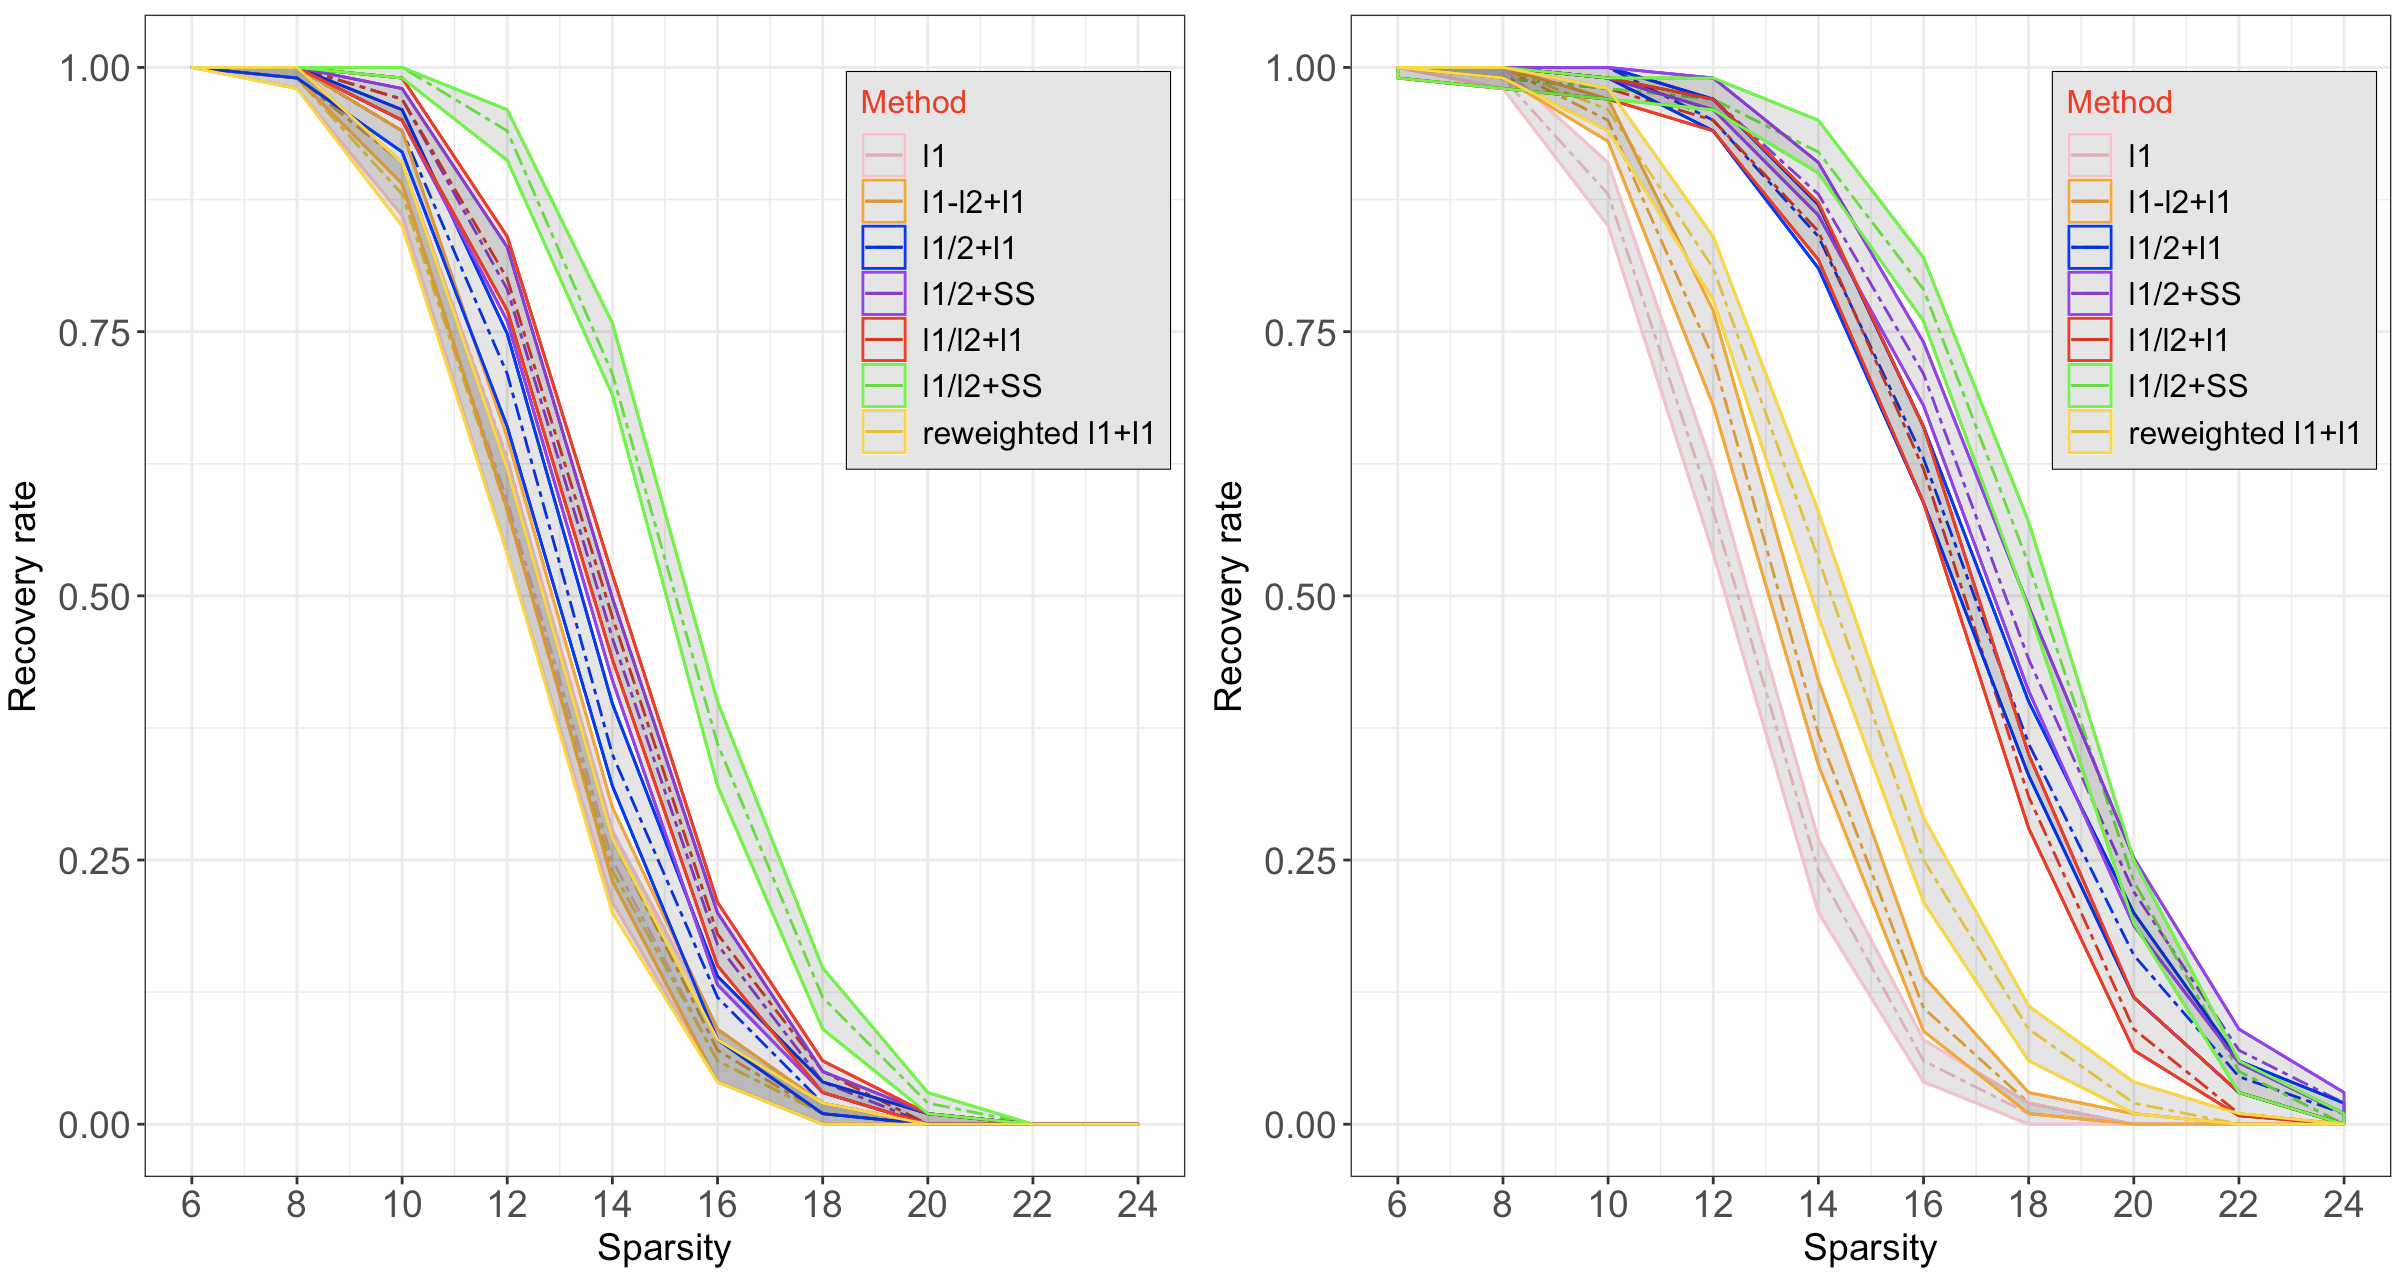
\includegraphics[width=11cm]{comparison1.png}
\caption{$0.2$-$0.5$-$0.8$ quantile plot of average recovery rate using $50\times 250$ gaussian random measurements: Unif$([-10, -5]\cup [5, 10])$ coefficients on the left and Unif$([-10, 10])$ coefficients on the right.}
\end{center}
\end{figure}


\end{frame}



\begin{frame}
\frametitle{Future directions}

\begin{itemize}

\item Study the theoretical aspects of the multi-dimensional version of $\ell_1/\ell_2$ in joint-sparse recovery, and the corresponding algorithms.

\medskip

\item The applications of the ratio-type penalties in other optimization problems.

\medskip

\item Other interesting questions arising from compressed sensing, matrix completion and sparse approximation. 

\end{itemize}


\end{frame}








\begin{frame}

Grateful for useful discussions with Tom Alberts, You-Cheng Chou, Akil Narayan and Dong Wang. 

\bigskip

\bigskip

\bigskip

\bigskip


{\begin{center} \large {\color{blue}Thanks! Questions?} \end{center}}


\end{frame}
\end{document}
